\section{Activation Functions}

\subsection{tanh}

Here is the formula for $tanh$: 
\begin{equation}
    \frac{e^x - e^{-x}}{e^x + e^{-x}}
\end{equation}

\begin{figure}[!htb]
    \centering
    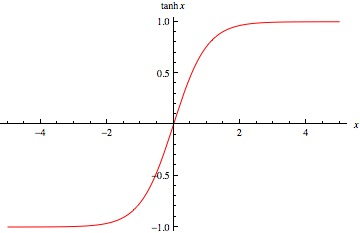
\includegraphics{images/TanhReal.jpg}
    \caption{$tanh$ Plot}
\end{figure}

And here is the derivative formula: 
\begin{equation}
    \frac{d tanh(x)}{dx} = sech^2(x) = \left( \frac{2}{e^x + e^{-x}} \right)^2
\end{equation}

\begin{figure}[!htb]
    \centering
    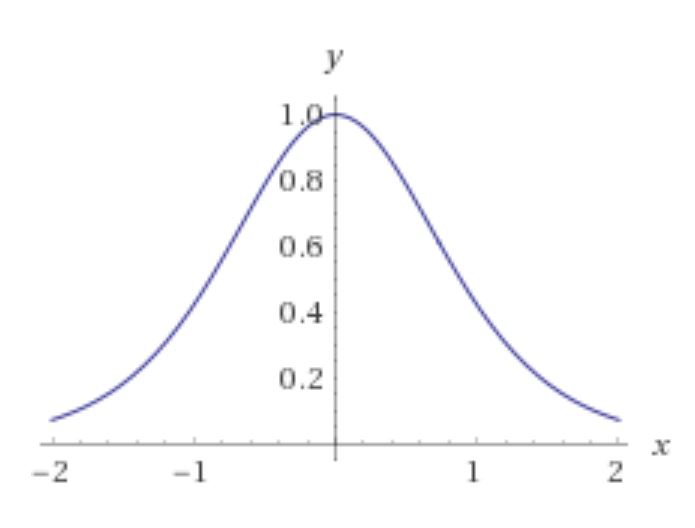
\includegraphics{images/tanhderivative.JPG}
    \caption{$tanh$ Derivative Plot}
\end{figure}

\subsection{Sigmoid}
Here is the formula for $\sigma$: 
\begin{equation}
    \sigma(x) = \frac{1}{1 + e^{-x}}
\end{equation}

\begin{figure}[!htb]
    \centering
    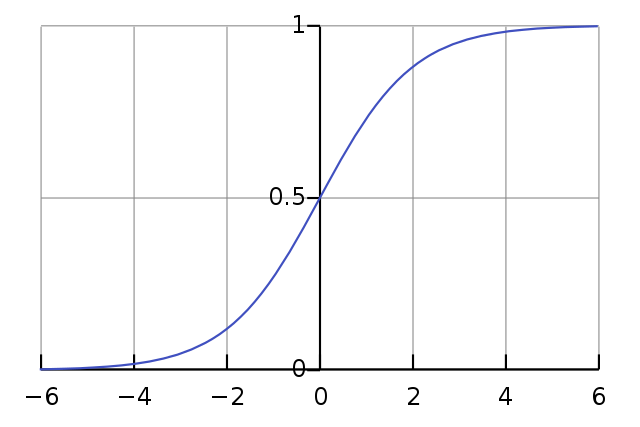
\includegraphics[scale=0.3]{images/640px-Logistic-curve.png}
    \caption{$\sigma(x)$ Plot}
\end{figure}

And here is the derivative formula: 
\begin{equation}
    \frac{d \sigma(x)}{dx} =  \frac{e^{-x}}{(1 + e^{-x})^2}
\end{equation}

\begin{figure}[!htb]
    \centering
    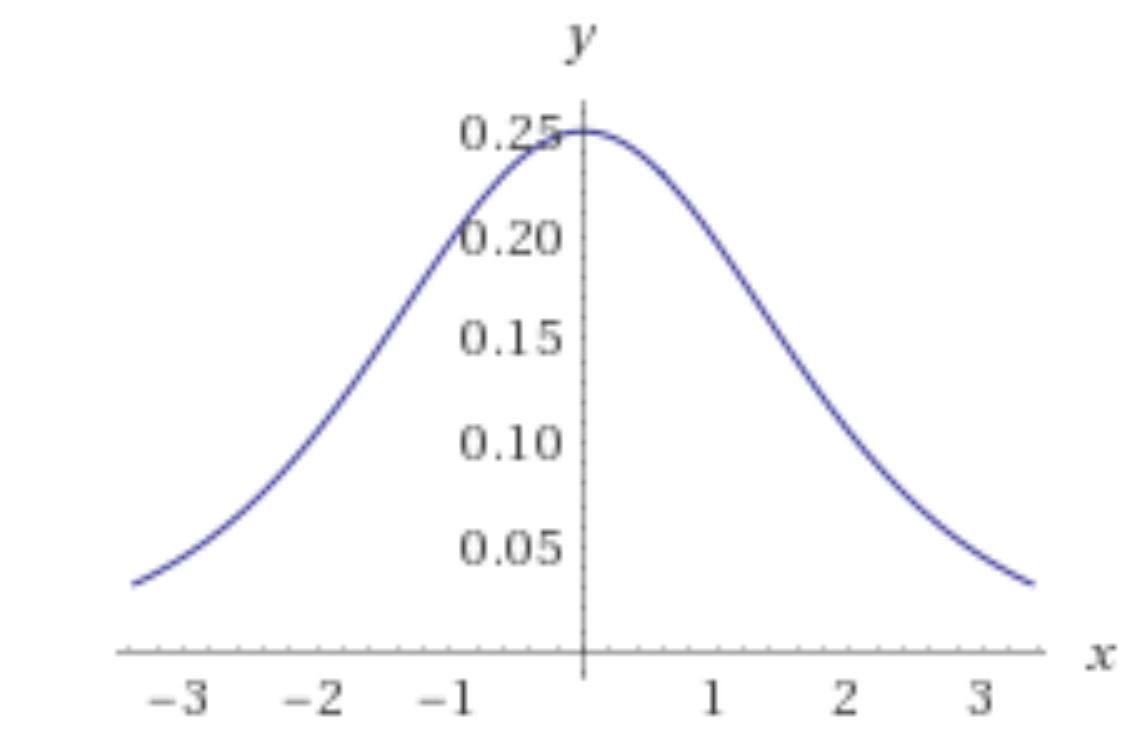
\includegraphics[scale=0.8]{images/sigmoidderivative.JPG}
    \caption{$\sigma(x)$ Derivative Plot}
\end{figure}

If we want to compare the above two functions $\sigma$ and $tanh$ it seems $tanh$ is preferred because it is symmetric around 0. Having data of a layer (even hidden layers) to be around zero helps more with training. because of this  also it is advised to have input data also normalized. Also having  zero mean inputs to a layer makes more sense on regularizations that we apply on the weights, otherwise the layers with non-zero mean input will suffer more from regularizations. See \cite{LeCun:1998:EB:645754.668382}

Another problem with all non-zero centred functions is that the force the gradient to have same polarity for it's elements. This will make the learning process very lengthy as the learning trajectory should be doubled at least. 

\section{ReLU}
Here is the formula for ReLU activation function. 

\begin{equation}
    f(x) = x^{+} = max(0, x)
\end{equation}

\begin{figure}[!htb]
    \centering
    \includegraphics[scale=0.3]{images/ReLU.jpg}
    \caption{ReLU Plot}
\end{figure}

The problem with ReLU is that is not derivativable. And we need to calculate the derivative for backpropagation training. So we need to come up with a close function to be derivativable. There are two options available either calculate the gradient by numerical method or estimate the function using an analytic function such a soft-ReLU. 
On the other hand there are multiple advantages associated with ReLU.  First of all it is more aligned with what we know from behaviour of biological neural systems. Also using ReLU activation function will result in  more sparse representations of the data. This is useful specially when the network is deep. In practice also it is performing better on pre-training models such Boltzmann Machines or deep belief networks. 

Also in ReLU as the output does not saturate, we have use some sort of regularization scheme to control the weight sizes. As one of the advantages of the ReLU unit is sparsity, it makes sense to use $L_1$ regularization which also promotes the sparsity. See \cite{pmlr-v15-glorot11a}

\subsection{Other Activation Functions}
We can name multiple activations functions compared to mentioned above: 
\begin{enumerate}
    \item  Leacky Relu: Instead of having flat left side for Relu we can impose a very small slope on it. So the function becomes $L(x) = max(\alpha x , x)$. We can also let the network to learn the slope of the negative part i.e. $\alpha$.  
    \item Softplus: Is analytic approximation of Relu. with formulation $f(x) = log( 1 + e^x)$. This function always have a derivative. The formula for the derivative of Softplus is logistic function $f^{\prime} = \frac{1}{1 + e^x}$. 
\end{enumerate}

\begin{figure}[!htb]
    \centering
    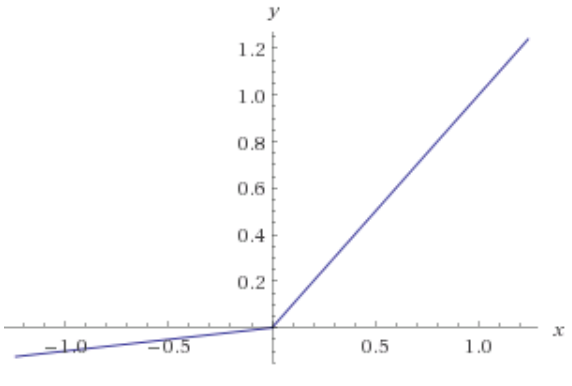
\includegraphics[scale=0.3]{images/leacky_relu.png}
    \caption{Leacky ReLU Plot}
\end{figure}

\begin{figure}[!htb]
    \centering
    \includegraphics[scale=0.3]{images/Softplus.png}
    \caption{Softplus Plot}
\end{figure}
